\documentclass[aps,amssymb,preprint,a4paper]{revtex4}
%\documentclass[aps,amssymb,a4paper,twocolumn]{revtex4}

%\usepackage[latin1]{inputenc}
\usepackage[T1]{fontenc}
\usepackage[english]{babel}
\usepackage{braket}
\usepackage{epsfig}
\usepackage{graphicx}
\usepackage{amsmath,amsfonts,amssymb}
\usepackage{dsfont}
\usepackage{booktabs}
\usepackage{units}
\usepackage{natbib}
\usepackage{xcolor}
\usepackage{multirow}
\usepackage{tikz,pgfplots}
%\usepackage{}
%\usepackage{}
%\usepackage{}

\usetikzlibrary{patterns,shadows,trees,calc}
\usepgfplotslibrary{units}

\pgfplotsset{compat=1.8}

\begin{document}


\newcommand{\wignerj}[6]{\mbox{$\left( \begin{array}{ccc} #1 & #2 & #3 \\ #4 & #5 & #6 \end{array} \right)$}}
\newcommand{\redume}[3]{\mbox{$( #1 || #2 || #3 )$}}

\setlength{\tabcolsep}{12pt}

% Define some colours
\definecolor{diplom1}{rgb}{0.0 0.4 1.0}
\definecolor{diplom2}{rgb}{0.0 0.0 0.6}
\definecolor{diplom3}{RGB}{153,0,0} %unirot

\title{Non-nearest Neighbour Interatomic Coulombic Decay}

\author{Elke Fasshauer}
\email[]{Email:Elke.Fasshauer@uit.no}


\affiliation{Centre for Theoretical and Computational Chemistry,
Department of Chemistry, University of Troms\o
-- The Arctic University of Norway, N-9037 Troms\o, Norway}

\date{\today}

%%%%%%%%%%%%%%%%%%%%%%%%%%%%%%%%%%%%%%%%%%%%%%%%%%%%%%%%
%                  Abstract                            %
%%%%%%%%%%%%%%%%%%%%%%%%%%%%%%%%%%%%%%%%%%%%%%%%%%%%%%%%
\begin{abstract}
Interatomic Coulombic Decay (ICD) is an electronic decay process of
excited, ionized systems. It has been shown to occur in a multitude of small
and large systems.
The effects of more than one possible decay
partner are discussed in detail illustrated by simulated ICD electron spectra
of NeAr clusters and pure Ne clusters.
Hereby, the mostly underestimated contribution of decay with
non-nearest neighbours is highlighted. In the neon clusters, the lifetime of the
bulk atoms is found to be in excellent agreement with experiment, while the
lifetimes of the surface atoms differ significantly. Hence, the experimental
lifetime can not purely be explained by the effect of the number of
neighbours.

We propose the possibility to investigate the transition from
small clusters to the solid state by using the ICD electron spectra to
distinguish between icosahedral and cuboctahedral cluster structures.
\end{abstract}


\maketitle


%%%%%%%%%%%%%%%%%%%%%%%%%%%%%%%%%
% Introduction
%%%%%%%%%%%%%%%%%%%%%%%%%%%%%%%%%
\section{Introduction}

The Interatomic Coulombic Decay (ICD) is an electronic decay process of an atom or
molecule (a unit) involving atoms or molecules of the environment. After an
ionization from the sub-valence region of a unit $A$, the vacancy is filled
by an electron of the same unit and the excess energy is transferred to a decay
partner $B$, which subsequently get ionized:

\begin{equation*}
 A^+ + B \rightarrow A^+ + B^+ + e^-_{ICD}  .
\end{equation*}

In the final state,
the two units $A$ and $B$ are both positively charged, repell each other and
thereby undergo a Coulomb explosion. This process was predicted theoretically
\cite{Cederbaum97} and later proven experimentally \cite{Marburger03}. Since then
it has been studied in a multitude of different systems such as small and large
rare gas clusters \cite{many,Fasshauer14_1},
clusters of small molecules \cite{},
quantum dots \cite{Bande13}
and proteins \cite{Harbach13}. Additionally it has given raise to
the investigation of a whole zoo of ICD-like processes (see Ref.
\cite{Hergenhahn11,Jahnke15}
and references therein).

In order to undergo ICD and this process to be observable, two criteria have to
be fulfilled: the energy and the coupling criterion. The energy criterion
requires the energy conservation to hold. In case the energy of the
doubly ionized final
state is higher than the energy of the singly ionized initial state, the ICD
is energetically forbidden. The coupling criterion requires the decay
process to be sufficiently efficient to outperform other decay pathways
such as radiative decay by emission of a photon or coupling to the nuclear
degrees of freedom in molecules. The corresponding property is the
decay width $\Gamma = \frac{\hbar}{\tau}$, which is inversely proportional
to the lifetime $\tau$ and proportional to the decay rate $\frac{1}{\tau}$.

The ICD process was so far mostly discussed for the case of decay partners in
the direct vicinity, because the decay widths with decay partners further away
was considered to be negligible. Therefore, the decay was studied in clusters
up to 13 neon atoms considering the initial ionization of only the central
atom and not the other ones \cite{Santra01_3}. In this study, a higher than
linear dependence of the decay width on the number of neighbours was
observed. A linear dependence would be expected for equally decay partners
at equal distances from the initially ionized atom in the same environment.
Since the decay width in the asymptotic limit shows an 
$1/\omega^{4}_{vp}$-behaviour on the energy of the virtual photon, which
is decreased for a stabilized final state, this additional feature
can be related to
the better energetic stabilization of the doubly ionized
final state in larger clusters \cite{Fasshauer13}.

We showed that decay pathways with decay partners at larger distances need to
be included for larger systems for two reasons:
\begin{enumerate}
 \item In cluster structures more than one pair of units can consist of
       the same atom types and have the same interatomic distance. Hence,
       they are indistinguishable in the spectrum. Since the decay rate
       as well as the peak intensity
       is proportional to the number of such pairs,
       the peaks stemming from several pairs are favoured
       compared to other ones at similar distances. Therefore, peaks
       stemming from decays with distant decay partners can be visible
       in ICD spectra of clusters. \cite{Fasshauer14_1}
 \item The opening of ICD-like decay channels depend on the interatomic
       distance. A channel being closed at the distance to the most direct
       neighbours might be open for interaction partners at slightly
       larger distances. If this particular decay channel is more efficient
       than other decay channels being open for the decay with direct
       neighbours, it can still be visible in the spectrum or even
       outperform the slower decay mechanism and hence they have to be
       taken into account. We have shown this for the case of ICD vs.
       the Electron Transfer Mediated Decay (ETMD3) process in mixed ArXe
       clusters \cite{Fasshauer13,Fasshauer16_1}.
\end{enumerate}
However, this feature of non-nearest neighbour ICD
has so far not been addressed by itself and we will fill the gap in this
paper.

For a test system we choose rare gas clusters are. These are favourable
for the investigation of basic features both
from a theoretical and an experimental point of view. Their spherical
symmetry and their very localized orbitals allow for an comparably easy
theoretical description of the decay processes and the gaseous state
of their components allows for a convenient cleaning of the experimental
setup allowing for higher count rates and therefore a higher resolution
of the spectra. At the same time, the structure of the clusters reveals an
interesting matter of research. Small, ideal clusters exhibit an icosahedral
structure while large clusters have a cuboctahedral structure, which
infinitely extended, yields the solid state face-centered-cubic (fcc) structure.
In the solid state, every single atom is surrounded by twelve other atoms in the
same distance. Surface atoms or even atoms at edges and vertices are rare
compared to the number of atoms in the bulk. 
These atoms being surrounded
However, in small clusters most atoms are surface atoms and are therefore
surrounded by less than the optimal 12 atoms.
In the icosahedral cluster structure the interatomic distance between different
layers are shorter than between atoms of the same layer. 
Therefore,
this structure is favourable in small clusters with a large surface-to-bulk ratio.
Together with the structure change from icosahedral to cuboctahedral
the clusters' properties gradually change towards those of solids and
conductivity as well as magnetizability can be observed. \cite{Benfield92}
It is still unclear at which cluster size the favourable structures changes from
an icosahedral to an cuboctahedral structure. Numbers in the range
of 800--3000 atoms have been reported. \cite{Hartke02,Pahl08}
We propose to use the ICD to be a possible tool to differentiate between
icosahedral and fcc cluster structures using the different distance
patterns in the cluster structures.

We will
therefore first introduce the theoretical concepts in section \ref{sec:theory},
present the computational details in section \ref{sec:computational},
discuss the distance dependency of the ICD in general
in section \ref{sec:partners} and then
zoom in on the NeNe ICD part of the ICD spectra of NeAr clusters
\cite{Fasshauer14_1} in section \ref{sec:near}. Here we will discuss the
peaks and their origin in detail and thereby
raise the question, what a \emph{nearest neighbour} is supposed to be. From
our conclusions we propose the possibility to distinguish cluster structures
of ideal icosahedral and cuboctahedral structures using ICD spectra in
section \ref{sec:icofcc}.

%\begin{figure}[h]
% \centering
% \includegraphics[width=\columnwidth]{pics/2dim_coincs.eps}\\
% 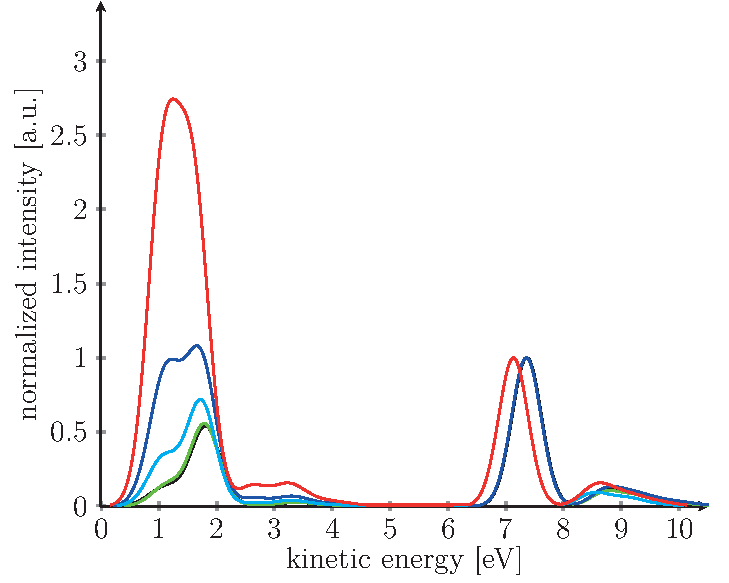
\includegraphics[width=\columnwidth]{pics/NeArcluster_theospecs.pdf}
% \caption{Experimental and theoretical NeAr ICD spectra \cite{Fasshauer14_1}.
%          The experimental spectra were obtained for different cluster expansion
%          conditions and the theoretical spectra were obtained for different
%          underlying cluster structures. In both the NeNe and the NeAr ICD part
%          of the spectrum a main peak and next to it at least one more peak at
%          higher energies are observed. These smaller peaks stem from decays
%          with decay partners at larger distances \cite{Fasshauer13,Fasshauer14_1}.}
% \label{figure:near_spectra}
%\end{figure}


%%%%%%%%%%%%%%%%%%%%%%%%%%%%%%%%%%%%%%%%%%%%%%%%%%%%
%%%%%%%%%  Theory
%%%%%%%%%%%%%%%%%%%%%%%%%%%%%%%%%%%%%%%%%%%%%%%%%%%%
\section{Theoretical Background}
\label{sec:theory}

In roder to simulate the ICD electron spectra for a given cluster structure,
the kinetic energies of the ICD electrons $E_{ICD}$ and the corresponding decay
decay widths of all pairs have to be determined. The ICD electron energies
are given by the differences between the initial state and the final state
energies $E_{in}$ and $E_{fin}$, respectively. The initial state energy
is given by the single ionization potential (SIP) of the sub-valence electron
of the entire system
and the final state energy is given by the double ionization potential (DIP).
In the asymptotic limit, which is a reasonably good approximation for
weakly bound systems, he initial state energy is approximated by the SIP
of the initially ionized unit $X_{in}$ and the final state energy can be
approximated
by the sum over the SIPs of the electron donating unit $X_D$ and the electron
emitting unit $X_E$ ionized in the final state as well as the
Coulomb repulsion between two point charges at the interatomic distance $R$

\begin{align}
 E_{ICD}^\beta &= E_{in}^\beta - E_{fin}^\beta \label{equation:E_sec}\\
 E_{in}        &= SIP(X_{in}) \label{equation:E_in}\\          
 E_{fin}^\beta &= SIP(X_{D}^\beta) + SIP(X_{E}^\beta) + \frac 1R
           \label{equation:E_fin}                . 
\end{align}
Here, $\beta$ denotes the selected decay channel.

Following Wentzel \cite{Wentzel27}, Feshbach\cite{Feshbach58,Feshbach62}
and Fano \cite{Fano61} the decay width is given by

\begin{equation}
 \Gamma_{\beta}(E_{res}) = 2\pi \left|
                           \braket{\Phi_{in}| H_f |\chi_{\beta}}
                           \right|^2   .
\end{equation}
Here, the bound and ionized initial state is described by $\ket{\Phi_{in}}$ and
the final continuum state of a particular decay channel $\beta$ is
given by $\ket{\chi_{\beta}}$.
Its challenging description involving both bound and continuum states can
amongst others be achieved by the FanoADC-Stieltjes approach, where a
subset of the $2h1p$ functions within the Algebraic Diagrammatic Construction
(ADC) are used to mimic the final state function $\ket{\chi_{\beta}}$.
By these means calculated discrete energies and corresponding transitions
moments are then used to construct a continuous function, which is evaluated
at the resonance energy approximated by the single ionization potential
corresponding to the initial state $E_{in}$. For a more detailed
description of the method and comparison to other approaches see References
\cite{Averbukh05,Fasshauer15_1} and references therein.


%%%%%%%%%%%%%%%%%%%%%%%%%%%%%%%%%%%%%%%%%%%%%%%%%%%%
%%%%%%%%%  Computational Details
%%%%%%%%%%%%%%%%%%%%%%%%%%%%%%%%%%%%%%%%%%%%%%%%%%%%
\section{Computational Details}
\label{sec:computational}
The cluster structures used were constructed to have an ideal icosahedral or
face-centered-cubic geometry with optional additional incomplete outermost
shells. These are based on the van der Waals radii for neon
$r_{Ne}=$ \unit[1.54]{\AA}
and argon $r_{Ar}=$ \unit[1.88]{\AA} \cite{Bondi64}.
In case of the NeAr clusters two of those
cluster structures from Ref. \cite{Fasshauer14_1}, where the theoretical
and experimental argon content in the cluster,
the NeAr-ICD to total
ICD ratio and the peak position of the NeAr-ICD peak matched best for a given
manifold (set) of clusters produced under certain experimental conditions,
have been chosen.
These are $C_{Ar}=3$, $C_{Ne}=1$, $S_{Ne}=7$ for set 3
and $C_{Ar}=2$, $C_{Ne}=1$, $S_{Ne}=13$ for set 5 where we used the same
nomenclature as in Ref. \cite{Fasshauer14_1}. Hence, $C_{Ar}$ denotes
the edge length of the argon core, $C_{Ne}$ denotes the number of complete
neon shells around the argon core and $S_{Ne}$ denotes the number of 
triangular surfaces additionally covered by neon atoms.


\begin{table}[h]
 \caption{Experimental values for the single ionization potentials
          \cite{Fasshauer14_1}
          used for the estimation of the decay widths.}
 \label{table:exp_input}
 \centering
 \begin{tabular}{lc}
  \toprule
  indicator            &  value \\
  \midrule
  SIP(Ne2s)            &  \unit[47.75]{eV} \\
  SIP(Ne2p)            &  \unit[21.10]{eV} \\
  SIP(Ar3p)$_{c<3}$    &  \unit[15.40]{eV} \\
  SIP(Ar3p)$_{c\ge 3}$ &  \unit[15.20]{eV} \\
  \bottomrule
 \end{tabular}
\end{table}


The calculations to obtain the ICD electron spectra of all cluster
structures were performed with
the program HARDRoC \cite{HARDRoC} based on the decomposition of the cluster into
pairs. Every pair with the same distance is treated equally. This includes the
assumption that every neon atom is ionized with the same probability.
\cite{Fasshauer14_1,Fasshauer_thesis}
It uses experimental ionization energies shown
in Table \ref{table:exp_input} and curves fitted to the decay width of the
NeNe ICD of Ref. \cite{Averbukh06_1} and the NeAr decay widths of Ref.
\cite{Fasshauer14_1}. These fitted curves yield lifetimes
$\tau=\frac{\hbar}{\Gamma}$ at the corresponding equilibrium distances of
$\tau_{NeNe}= \unit[60]{fs}$ and
$\tau_{NeAr}= \unit[44]{fs}$.


%%%%%%%%%%%%%%%%%%%%%%%%%%%%%%%%%%%%%%%%%%%%%%%%%%%%
%%%%%%%%%  Results and discussion
%%%%%%%%%%%%%%%%%%%%%%%%%%%%%%%%%%%%%%%%%%%%%%%%%%%%
\section{Decay with Decay Partners at Different Distances}
\label{sec:partners}

To fully understand the spectra of clusters with several possible
initially ionized atoms with multiple decay partners it is necessary to
understand the properties of the decay of a single pair of atoms. As can be seen
from Eqs. (\ref{equation:E_sec}) -- (\ref{equation:E_fin}),
the kinetic energy of the ICD electron follows an
$1/R$-behaviour shown in Figure \ref{figure:model_RE} for the case
of a neon dimer at different distances.

\begin{figure}[h]
 \centering
 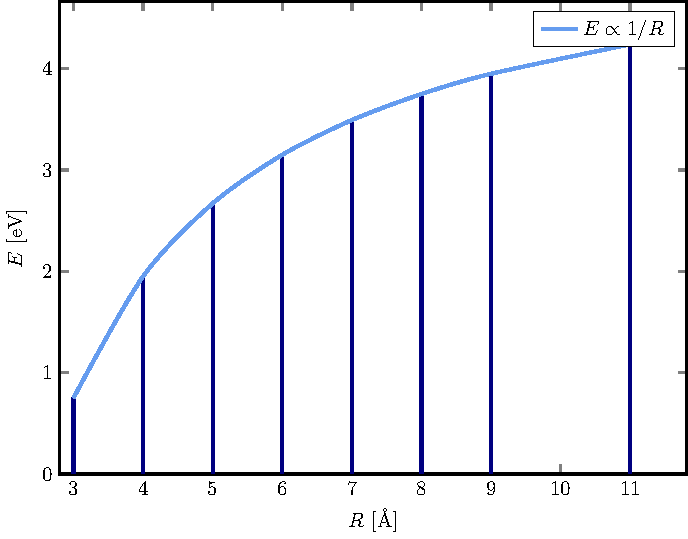
\includegraphics[width=\columnwidth]{pics/model_RE.pdf}
 \caption{Kinetic energy of the ICD electron depending on the interatomic
          distance of the two atoms involved in the decay within the
          asymptotic approximation. The kinetic energy shows a $1/R$
          behaviour and hence distance changes at small distances lead
          to larger changes in the kinetic energy than at larger distances.}
 \label{figure:model_RE}
\end{figure}
From this diagram it can already be
seen that the kinetic energies stemming from equidistant peaks of
\unit[3]{\AA}, \unit[4]{\AA}, \unit[5]{\AA}, \dots ,\unit[9]{\AA} are
not equidistant in their energy difference but rather decrease for
an increasing interatomic distance.

The corresponding decay widths $\Gamma$ depending on the interatomic
distance are shown in Figure \ref{figure:model_RGamma}. They show an
asymptotic $1/R^6$-behaviour such that the decay widths from an interatomic
distance of \unit[7]{\AA} on are too small to be seen in the
figure. This means that in case of a neon dimer with an internuclear distance
of \unit[3]{\AA}, a decay with one decay partner at twice the internuclear
distance of the neon dimer is very unlikely, but that interactions with
decay partners at shorter distances can not in general be neglected.

\begin{figure}[h]
 \centering
 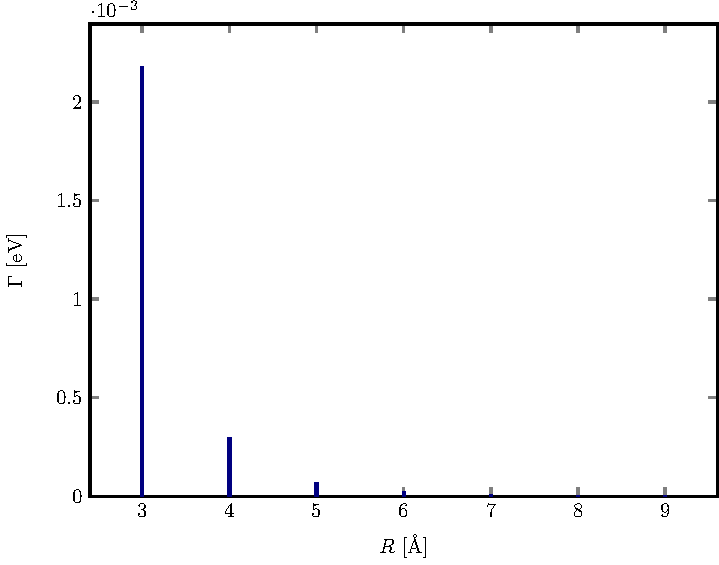
\includegraphics[width=\columnwidth]{pics/model_RGamma.pdf}
 \caption{Decay widths for different interatomic distances following an
          asymptotic $1/R^6$-behaviour. For distances larger than twice
          the shortest distance considered the peaks are not visible in this
          plot.}
 \label{figure:model_RGamma}
\end{figure}

A similar picture is given by the hypothetical ICD-electron spectrum for
decay partners at distances of \unit[3]{\AA}, \unit[4]{\AA}, \dots,
\unit[9]{\AA} shown in Figure \ref{figure:model_EGamma}. Here, the kinetic
energy of the ICD electron is depicted on the abscissae while the decay
width $\Gamma$ is plotted on the ordinate. Since the decay width is proportional
to the decay rate and hence the decay propability, these spectra can directly
be compared to experimental ICD electron spectra.

\begin{figure}[h]
 \centering
 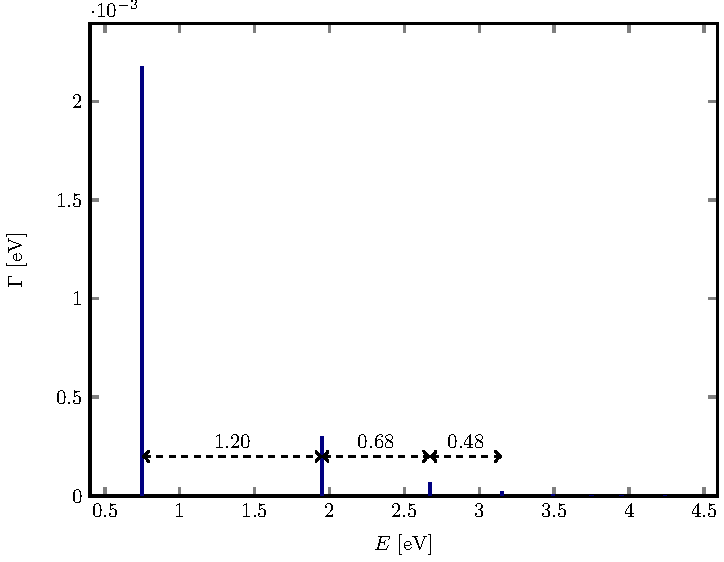
\includegraphics[width=\columnwidth]{pics/model_EGamma.pdf}
 \caption{ICD electron spectrum for interaction partner distances of
          \unit[3]{\AA}, \unit[4]{\AA}, \unit[5]{\AA}, \dots ,\unit[9]{\AA}.
          The energy difference between equidistant interaction partners
          decreases with increasing distance. For the case of Ne$_2$ pairs
          these energy differences between the peaks stemming from different
          interatomic distances are given by:
          \unit[3]{\AA},\unit[4]{\AA} $\rightarrow$ \unit[1.20]{eV},
          \unit[4]{\AA},\unit[5]{\AA} $\rightarrow$ \unit[0.68]{eV} and
          \unit[5]{\AA},\unit[6]{\AA} $\rightarrow$ \unit[0.48]{eV}.
          This means that the spectrum is better resolved for smaller distances
          and that small distance changes like vibrations will mainly affect
          this lower energy part of the spectrum.
}
 \label{figure:model_EGamma}
\end{figure}

The first and dominant peak stems from the decay with a decay
partner at a distance of \unit[3]{\AA}. The energy distance to the next peak
stemming from a decay with a decay partner with an internuclear distance of
\unit[4]{\AA} is found at a \unit[1.20]{eV} higher kinetic energy and the
energy difference to the next peak stemming from a \unit[5]{\AA} distant
decay partner is further \unit[0.68]{eV} higher. The increase of kinetic
energy of the ICD electron is caused by a decrease of Coulomb repulsion between
the interaction partners in the final state and therefore, the additional
excess in energy is converted into kinetic energy of the emitted ICD electron.
The energy difference between the peaks shown in Figure \ref{figure:model_EGamma}
decreases with an increasing distance of decay partners and at the same time
the kinetic energy
of the ICD electron. This means that for smaller interatomic distances and
comparably low kinetic energies of the ICD electron, the spectrum has a higher
resolution.
Therefore, a peak structure might be visible for the decay with nearest
neighbours (or the closest atoms with energetically allowed decay channels)
but not necessarily for all different kinds of interaction partners at larger
distances.

%\begin{figure}
% \centering
% \includegraphics[width=\textwidth]{pics/}
% \caption{}
% \label{}
%\end{figure}

\section{ICD in Clusters}

\subsection{NeAr Clusters}
\begin{figure}[h]
 \centering
 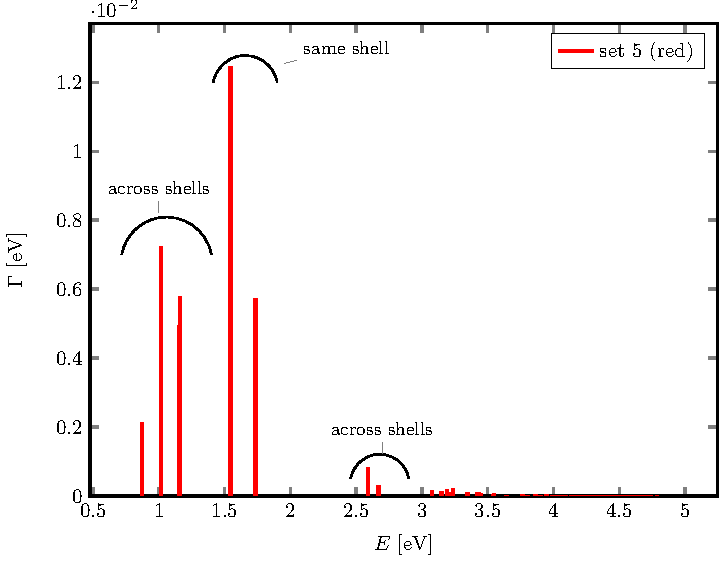
\includegraphics[width=\columnwidth]{pics/rot.pdf}\\
 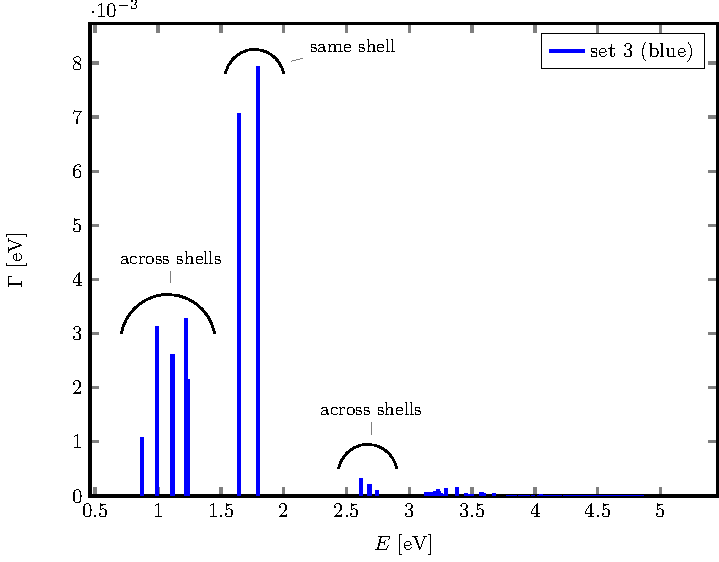
\includegraphics[width=\columnwidth]{pics/blue.pdf}
 \caption{ICD spectra for the NeNe-ICD part of the structures of set 3 and
          set 5 of the NeAr clusters in Ref. \cite{Fasshauer14_1}
          plotted as stick spectra.
          The different peak groups resemble different pair types
          within the NeAr clusters. The lowest energy peaks (\textbf{a})
          refer to nearest neighbours
          of different shells, the peak group \textbf{b} refers
          to nearest neighbours within one shell and the peak group \textbf{c}
          refers to next nearest neighbours between different shells.
          The peaks in group \textbf{d} contain both peaks stemming from
          pairs within the same shell as well as pairs consisting of atoms
          of different shells.}
 \label{figure:rot}
\end{figure}

%\begin{figure}
% \centering
% 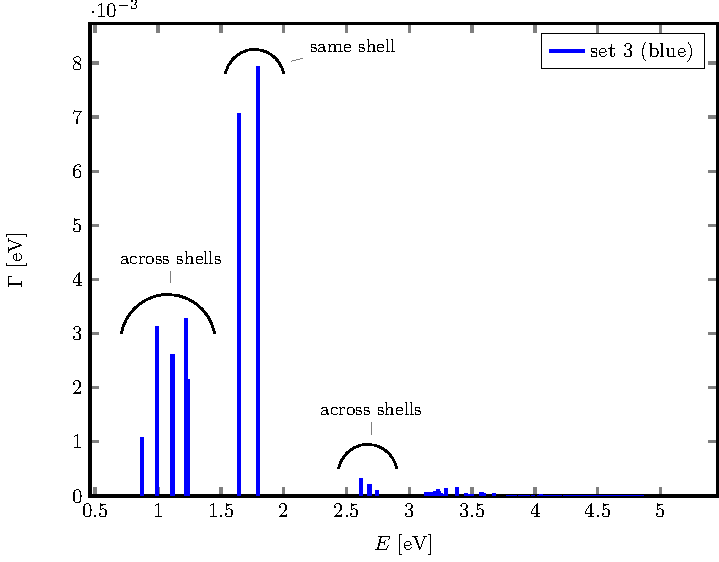
\includegraphics[width=\textwidth]{pics/blue.pdf}
% \caption{}
% \label{figure:blue}
%\end{figure}

\subsection{Icosahedral vs. fcc Structure of Clusters}
\begin{figure}[h]
 \centering
 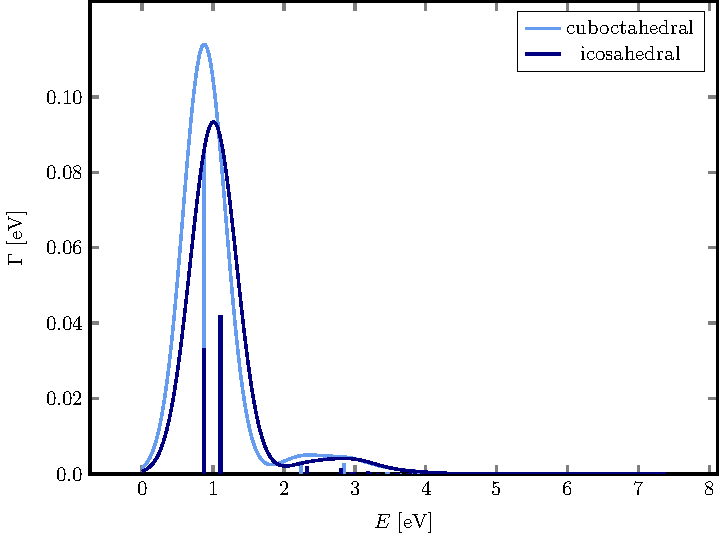
\includegraphics[width=\columnwidth]{pics/reinNe}
 \caption{ICD spectra of pure neon clusters consisting of 55 atoms in
          icosahedral and fcc structure. In clusters with an ideal fcc structure
          all interatomic distances are the same and hence only one peak
          for each shell around any atom in the cluster is to be expected.
          In ideal icosahedral clusters the interatomic distances between atoms
          within the same shell and between atoms in neighbouring atoms
          are different. Therefore two peaks for interactions partners
          at different distances can be expected. This feature might
          help to experimentally identify the underlying structure of clusters.}
 \label{figure:reinNe}
\end{figure}


%%%%%%%%%%%%%%%%%%%%%%%%%%%%%%%%%%%%%%%%%%%%%%%%%%%%
%%%%%%%%%  Conclusions
%%%%%%%%%%%%%%%%%%%%%%%%%%%%%%%%%%%%%%%%%%%%%%%%%%%%
\section{Summary}
\label{sec:summary}

We have discussed two of the three aspects one needs to take into account
to simulate the ICD spectrum of rare gas clusters in detail. Due to the nature
of clusters, a neon atom ionized in the inner-valence will have several decay
partners at different distances. The larger the interatomic distance the higher
is the kinetic energy of the ICD electrons which will yield a multitude of
peaks in the spectrum. These are then weighted by the decay width, which
depends on the interatomic distance of the decay partners but also needs
to be scaled by the number of pairs of the same distance.
The manifold of all different decay events will then yield the spectrum.

When applying these apsects to cluster structures, one finds that not only
the nearest neighbours contribute to the spectrum, but several other decay
partners do as well. Decay partners until a distance of at least twice the
distance of the clostest decay partners should be taken into account.
In clusters with an icosahedral cluster structure this is especially important
because the smallest interatomic distance between atoms of the same and atoms
of different layers is different, but both distances are comparable.
This leads to a different number of peaks in the spectra which might help to
differentiate between clusters of icosahedral and cuboctahedral cluster structure.

\ack

%\begin{acknowledgements}
Funding from the Research
Council of Norway through a Centre of Excellence Grant (Grant No.\ 179568/V30)
is gratefully acknowledged.
%\end{acknowledgements}


\clearpage

\bibliographystyle{apsrev4-1}
\bibliography{theolit}

\end{document}
